\chapter{System Analysis and Design}
\label{ch:system_analysis}

\section{Overview}
The \textbf{Legal Precedent Assistant for Indian Family Courts} project aims to provide a highly accurate modular and transferrable NLP model for ILC. 
The proposed model will be built for Family courts and use Legal-BERT and Llama 3 as baselinses with DAPT for both models on ILC. 
This chapter presents a comprehensive analysis of requirements, constraints, design alternatives, and system architecture that directly address the research gaps and problem statement identified in Chapters~\ref{ch:intro} and~\ref{ch:lit_review}.

\section{Requirements Analysis}

\subsection{Functional Requirements}
Based on the identified research gaps and Legal professional's needs, the system must fulfill the following functional requirements:

\textbf{FR1: Legal Document Input}
\begin{itemize}
    \item The legal documents/summaries from both sides should be given as input to the system alongside any pre-existing court judgements/summaries.
    \item The files can be uploaded as .docx/.pdf/.txt formats.
\end{itemize}

\textbf{FR2: Text Cleaning and Preprocessing}
\begin{itemize}
    \item The system pipeline will then use regex/BERT models to remove any unnecessary symbols and patterns to convert the input documents into text files for further processing.
\end{itemize}

\textbf{FR3: Evidence Scrutinization}
\begin{itemize}
    \item Llama 3.1 should be used to perform evidence scrutinization and a consistency audit for both sides, to try and determine contradictions in both side’s statements.
\end{itemize}

\textbf{FR4: IPC Mapping}
\begin{itemize}
    \item If the document contains any articles/code/IPC violations they should be tracked either based on the codes or based on statements.
\end{itemize}

\textbf{FR5: Precedent Retrieval}
\begin{itemize}
    \item Match the current court case documents with past similar court cases and find precedents from past judgements to aid in verdict/judgement of present case.
\end{itemize}

\textbf{FR6: Verdict Prediction}
\begin{itemize}
	\item Predict the verdict using the previous 3 requirements.

\end{itemize}

\textbf{FR7: Summarization}
\begin{itemize}
	\item •	Summarize the judgement and the case contents in 150 words or less.

\end{itemize}

\subsection{Non-Functional Requirements}

\textbf{NFR1: Cost Effectiveness}
\begin{itemize}
    \item Make use of freely available datasets and LLM models.
\end{itemize}

\textbf{NFR2: Usability and Accessibility}
\begin{itemize}
    \item The system should be easy to use and understand not just for Legal professionals, but also laymen.
\end{itemize}

\textbf{NFR3: Reliability and Maintainability}
\begin{itemize}
    \item The system should be able to handle any cases in the Family courts domain reliably, and should be maintained and upgraded as per changes in Family law. 
\end{itemize}

\textbf{NFR4: Explainability and Interpretability}
\begin{itemize}
    \item The verdicts/judgements/summaries should be explained and sources for precedents should be cited.
\end{itemize}

\textbf{NFR5:  Scalability and Extensibility}
\begin{itemize}
	\item The model should be expandable to other domains such as IP and Copyright laws, Criminal laws, Civil suits, etc.
\end{itemize}


\section{Constraints and Design Trade-offs}

\subsection{Hardware Constraints}
\textbf{C1: GPU requirements}
\begin{itemize}
    \item The current device uses a Notebook version of GTX 1650 gpu with 4Gb of VRAM.
    \item This is sufficient to train smaller BERT/LLM models with small batch size but takes longer times and has low efficiency.
    \item Solution: More advanced GPUs such as RTX series, or Ampere architecture based GPUs might be required based on the dataset procured.
\end{itemize}

\textbf{C2: VRAM/Memory Requirements}
\begin{itemize}
    \item The current device; GTX 1650 GPU has 4GB of VRAM, which is sufficient to train small to medium size BERT models provided Batching is used.
    \item Solution: However, for LLMs like Llama 3 and above, we might require over 12GB of VRAM which is consequently tied to the GPU.
    \item Solution: If powerful GPUs are not available, we can use CPU RAM as swap space/shared memory given that the project is being run on a Linux kernel.
\end{itemize}




\subsection{Software and Performance Constraints}
\textbf{C3: 512 token limit on BERT}
\begin{itemize}
    \item LegalBERT and its contemporaries have a strict 512 token limit.
    \item Solution: This limit can be circumvented by using Sliding sequence window technique.
\end{itemize}

\textbf{C4: Overfitting}
\begin{itemize}
    \item Overfitting happens often due to small size of datasets and low variety in data.
    \item Solution: Overfitting can be overcome by using DAPT, Contrastive Learning, Regularization and Early stopping.
\end{itemize}

\textbf{C5: Synthetic Data}
\begin{itemize}
	\item Synthetic data can help augment the size and balancer of dataset but can lead to outputs that are not representative of real life scenarios.
	\item Solution: Use minimal amounts of synthetic data and only for classes that have no instances at all.
\end{itemize}

\textbf{C6: Closed loop bias}
\begin{itemize}
	\item Closed loop bias happens in RAGs and models using Synthetic data as the model reuses its own output for training.
	\item Solution: Can be overcome by building/acquiring a larger dataset and preventing/minimizing use of model output for training
\end{itemize}

\newpage

%\section{Design Alternatives and Justification}
%\subsection{VR Platform Selection}
%\textbf{Alternatives Considered:}
%\begin{enumerate}
%    \item \textbf{Valve Index + PC:} Pros: Superior FOV (130°), refresh rate (144 Hz), force feedback support. Cons: High cost (\$1000 headset + \$1500 PC), wired tethering limits mobility.
%    \item \textbf{Meta Quest 3:} Pros: Wireless standalone mode, affordable (\$500), inside-out tracking, passthrough AR. Cons: Lower processing power, 90 Hz max refresh rate.
%    \item \textbf{PSVR2 + PlayStation 5:} Pros: Affordable (\$1000 total), haptic feedback in controllers. Cons: Closed ecosystem, limited development flexibility.
%\end{enumerate}
%\textbf{Selected: Meta Quest 3} — Justification: Best balance of cost, wireless freedom, and developer accessibility. Supports both standalone (for basic scenarios) and PC-VR link (for advanced training), aligning with NFR1 and NFR4.
%
%\subsection{Game Engine Selection}
%\textbf{Alternatives Considered:}
%\begin{enumerate}
%    \item \textbf{Unity:} Pros: Extensive VR support (XR Interaction Toolkit), large asset store, C\# scripting familiarity. Cons: Less advanced default vehicle physics.
%    \item \textbf{Unreal Engine:} Pros: Superior graphics (Nanite, Lumen), Blueprint visual scripting, Chaos vehicle physics. Cons: Steeper learning curve, larger build sizes.
%    \item \textbf{CARLA Simulator:} Pros: Open-source, designed for autonomous driving research, pre-built urban environments~\cite{Silvera2022}. Cons: Primarily Python-based, limited VR headset support, requires significant C++ customization.
%\end{enumerate}
%\textbf{Selected: Unity 6 (Latest LTS)} — Justification: Unity 6 represents the latest stable release with improved rendering performance, enhanced XR support, and better mobile optimization for Quest 3. Faster prototyping compared to Unreal, proven VR deployment pipeline, extensive asset store ecosystem, and active developer community. Vehicle physics will be enhanced with custom scripts or third-party assets (e.g., Edy's Vehicle Physics, Realistic Car Controller). Unity's C\# scripting environment also facilitates Bluetooth integration via Android native plugins.
%
%\subsection{Control Input Architecture}
%\textbf{Alternatives Considered:}
%\begin{enumerate}
%    \item \textbf{Custom PCB with USB HID:} Pros: Lowest latency (<5ms), plug-and-play compatibility. Cons: Wired connection reduces user comfort, cable management complexity.
%    \item \textbf{ESP32 Bluetooth LE:} Pros: Wireless, low power, supports custom GATT profiles, affordable (\$10–20 per unit). Cons: 10–30ms latency, potential interference.
%    \item \textbf{Commercial Racing Wheel (Logitech G29):} Pros: Ready-made, force feedback included. Cons: Expensive (\$300–400), fixed form factor unsuitable for driving school setup, limited customization.
%\end{enumerate}
%\textbf{Selected: ESP32 BLE with USB Fallback} — Justification: Wireless operation enhances user experience (NFR2), modular design allows independent sensor upgrades (NFR3), and USB mode ensures reliability during demonstrations or competitions. Custom firmware enables latency optimization (<20ms achievable).

\section{System Objectives}
Based on the requirements analysis and design trade-offs, the system objectives are:
\begin{itemize}
    \item To design a modular, reliable and explainable Legal Precedent Assistant for Indian Family courts.
    \item To create a Pipeline that takes court documents from both the opposing sides as inputs, cleans and pre-processes them and passes them to later stages for creating outputs in line with the functional and non-functional requirements.
    \item To integrate LegalBERT for IPC mapping of any codes/articles/statements found in the input documents as well as retrieving legal precedents from past cases. 
    \item To integrate Llama 3 for evidence scrutinization, verdict prediction and summarization of given court documents.
    \item To create a system that can be transferred between different legal domains and not be constrained to just Family courts.
\end{itemize}

\newpage
\section{Comparative Analysis with Existing Solutions}

Table~\ref{tab:comparative_analysis} compares the proposed system against existing commercial and research VR driving simulators based on key design parameters derived from the requirements analysis.

\begin{table}[H]
\caption{Comparative analysis of VR driving simulator solutions}
\label{tab:comparative_analysis}
\centering
\small
\begin{tabular}{|p{3cm}|p{2.2cm}|p{2.2cm}|p{2.2cm}|p{2.2cm}|}
\hline
\textbf{Parameter} & \textbf{Proposed System} & \textbf{Legal-RAG \cite{b20}} & \textbf{Keynote-AI \cite{b15}} & \textbf{JurisCTC \cite{b14}} \\ \hline

Cost & NA & NA & NA & \$30 Million \\ \hline

Model/Framework & Llama 3 and Legal-BERT via DAPT & Llama 3 and RAG & BERT and DAPT & Adversarial BERT and UDA \\ \hline

Target Audience & Professionals and Laymen & Legal Professionals & Legal Professionals & Legal Professionals \\ \hline

Customizability & High & Low & High & High \\ \hline

Domain Transferability & High & Low & High & Medium \\ \hline

Interpretability & Low & Low & Low & Low \\ \hline

Language & English, Marathi, Hindi & Bangla, Arabic & Swedish, English, Norwegian & Mandarin \\ \hline

Customizability & High (modular design) & High (open-source) & Low (proprietary) & Low (vendor lock-in) \\ \hline

Regulatory Focus & RTO-aligned metrics & Research protocols & Entertainment & Commercial licensing \\ \hline

\end{tabular}
\end{table}

\textbf{Key Differentiators:}
\begin{itemize}
    \item \textbf{Affordability:} More afforadble as compared to professionally built systems.
    \item \textbf{Domain Specific:} One of the only LLMs that focuses on Indian Family courts data.
    \item \textbf{Transferrability:} Due to DAPT on Indian corpora, can be transferred to other court domains under Indian jurisdiction.
    \item \textbf{Accessibility:} Summarization module helps general public understand legal jargon by simplifying it.
\end{itemize}

\newpage

\section{System Components and Architecture}

The proposed system architecture consists of two integrated subsystems designed to address the functional requirements while respecting the identified constraints.

\subsection{Hardware Subsystem}
The physical control setup comprises:
\begin{itemize}
    \item \textbf{CPU:} Any processors such as intel i5/i7 12th gen and above or Ryzen 5/7 are usable.
    \item \textbf{GPU:} GTX 1650 or higher. RTX series GPUs with 12 GB VRAM or higher are preferred.
    \item \textbf{VRAM:} 4GB and higher.
\end{itemize}



\subsection{Software  Subsystem}

\begin{itemize}
    \item \textbf{Python 3.10:} Stable version with long term support and compatible with most hardware.
    \item \textbf{PyTorch CUDA:} For parallel computing to improve training and dataset pre-processing efficiency.
    \item \textbf{Legal-BERT: } For initial stages of the system such as IPC/sections mapping, Precedent finding, etc.
    \item \textbf{Llama 3:} For more complex stages such as Evidence scrutinization, Summarization, and Verdict prediction.
\end{itemize}



\newpage

\section{System Architecture Diagram}

Figure~\ref{fig:system_architecture} illustrates the data flow and component interactions within the LPA system.

\begin{figure}[H]
    \centering
    \includegraphics[width=0.6\textwidth]{figs/system_architecture.pdf}
    \caption{System architecture showing data flow from input documents through pre-processing/cleaning stages to contextual extraction and analysis stages.}
    \label{fig:system_architecture}
\end{figure}

%\begin{figure}[H]
%    \centering
%    \includegraphics[width=0.95\textwidth]{figs/model_diagram.pdf}
%    \caption{System model diagram illustrating the conceptual architecture and relationships between core system components.}
%    \label{fig:model_diagram}
%\end{figure}

\section{Design Rationale Summary}

The design decisions documented in this chapter directly address the research gaps identified in Section~\ref{sec:gap_analysis}:

\begin{itemize}
    \item \textbf{Gap 1 (Localized Context)} By training specifically on the Indian Legal Corpus (ILC) and incorporating IPC-specific logic, the model overcomes the "Geographic Bias" of existing systems that rely solely on US, EU, or Chinese legal data.
    \item \textbf{Gap 2 (Long Document Handling):} The implementation of Hierarchical Transformers (or sliding-window techniques) directly addresses the 512-token limit of standard BERT models, allowing for the processing of verbose Indian High Court and Supreme Court judgments.
    \item \textbf{Gap 4 (Resource Efficiency):} The use of Domain Adaptive Pre-Training (DAPT) on specialized legal data ensures that the model achieves high F1 gains (up to 18.2\%) while remaining computationally lighter and more affordable than massive, general-purpose LLMs.
    \item \textbf{Gap 5 (Multi-task Integration):} The architecture combines Verdict Prediction, Case Summarization, and Statute Identification into a single pipeline, solving the limitation of fragmented systems that focus only on isolated subtasks like charge prediction.
    \item \textbf{Gap 6 (Semantic Accuracy): }  By utilizing LegalBERT and Dual-Attention mechanisms, the system captures complex legal jargon and intra-sentence relationships that traditional "Bag of Words" or basic frequency models fail to retrieve.
\end{itemize}

The comparative analysis (Table~\ref{tab:comparative_analysis}) demonstrates that this design occupies a unique position: language flexibility, domain transferrability, efficient training at commercial-training affordability, specifically tailored for the Indian Legal landscape.

\newpage

\section{Workflow and Operational Flow}
The workflow diagram (Figure~\ref{fig:workflow}) shows the sequential process of system operation—from initialization through user interaction to post-session evaluation—illustrating how the system supports a complete training cycle.

\begin{figure}[H]
    \centering
    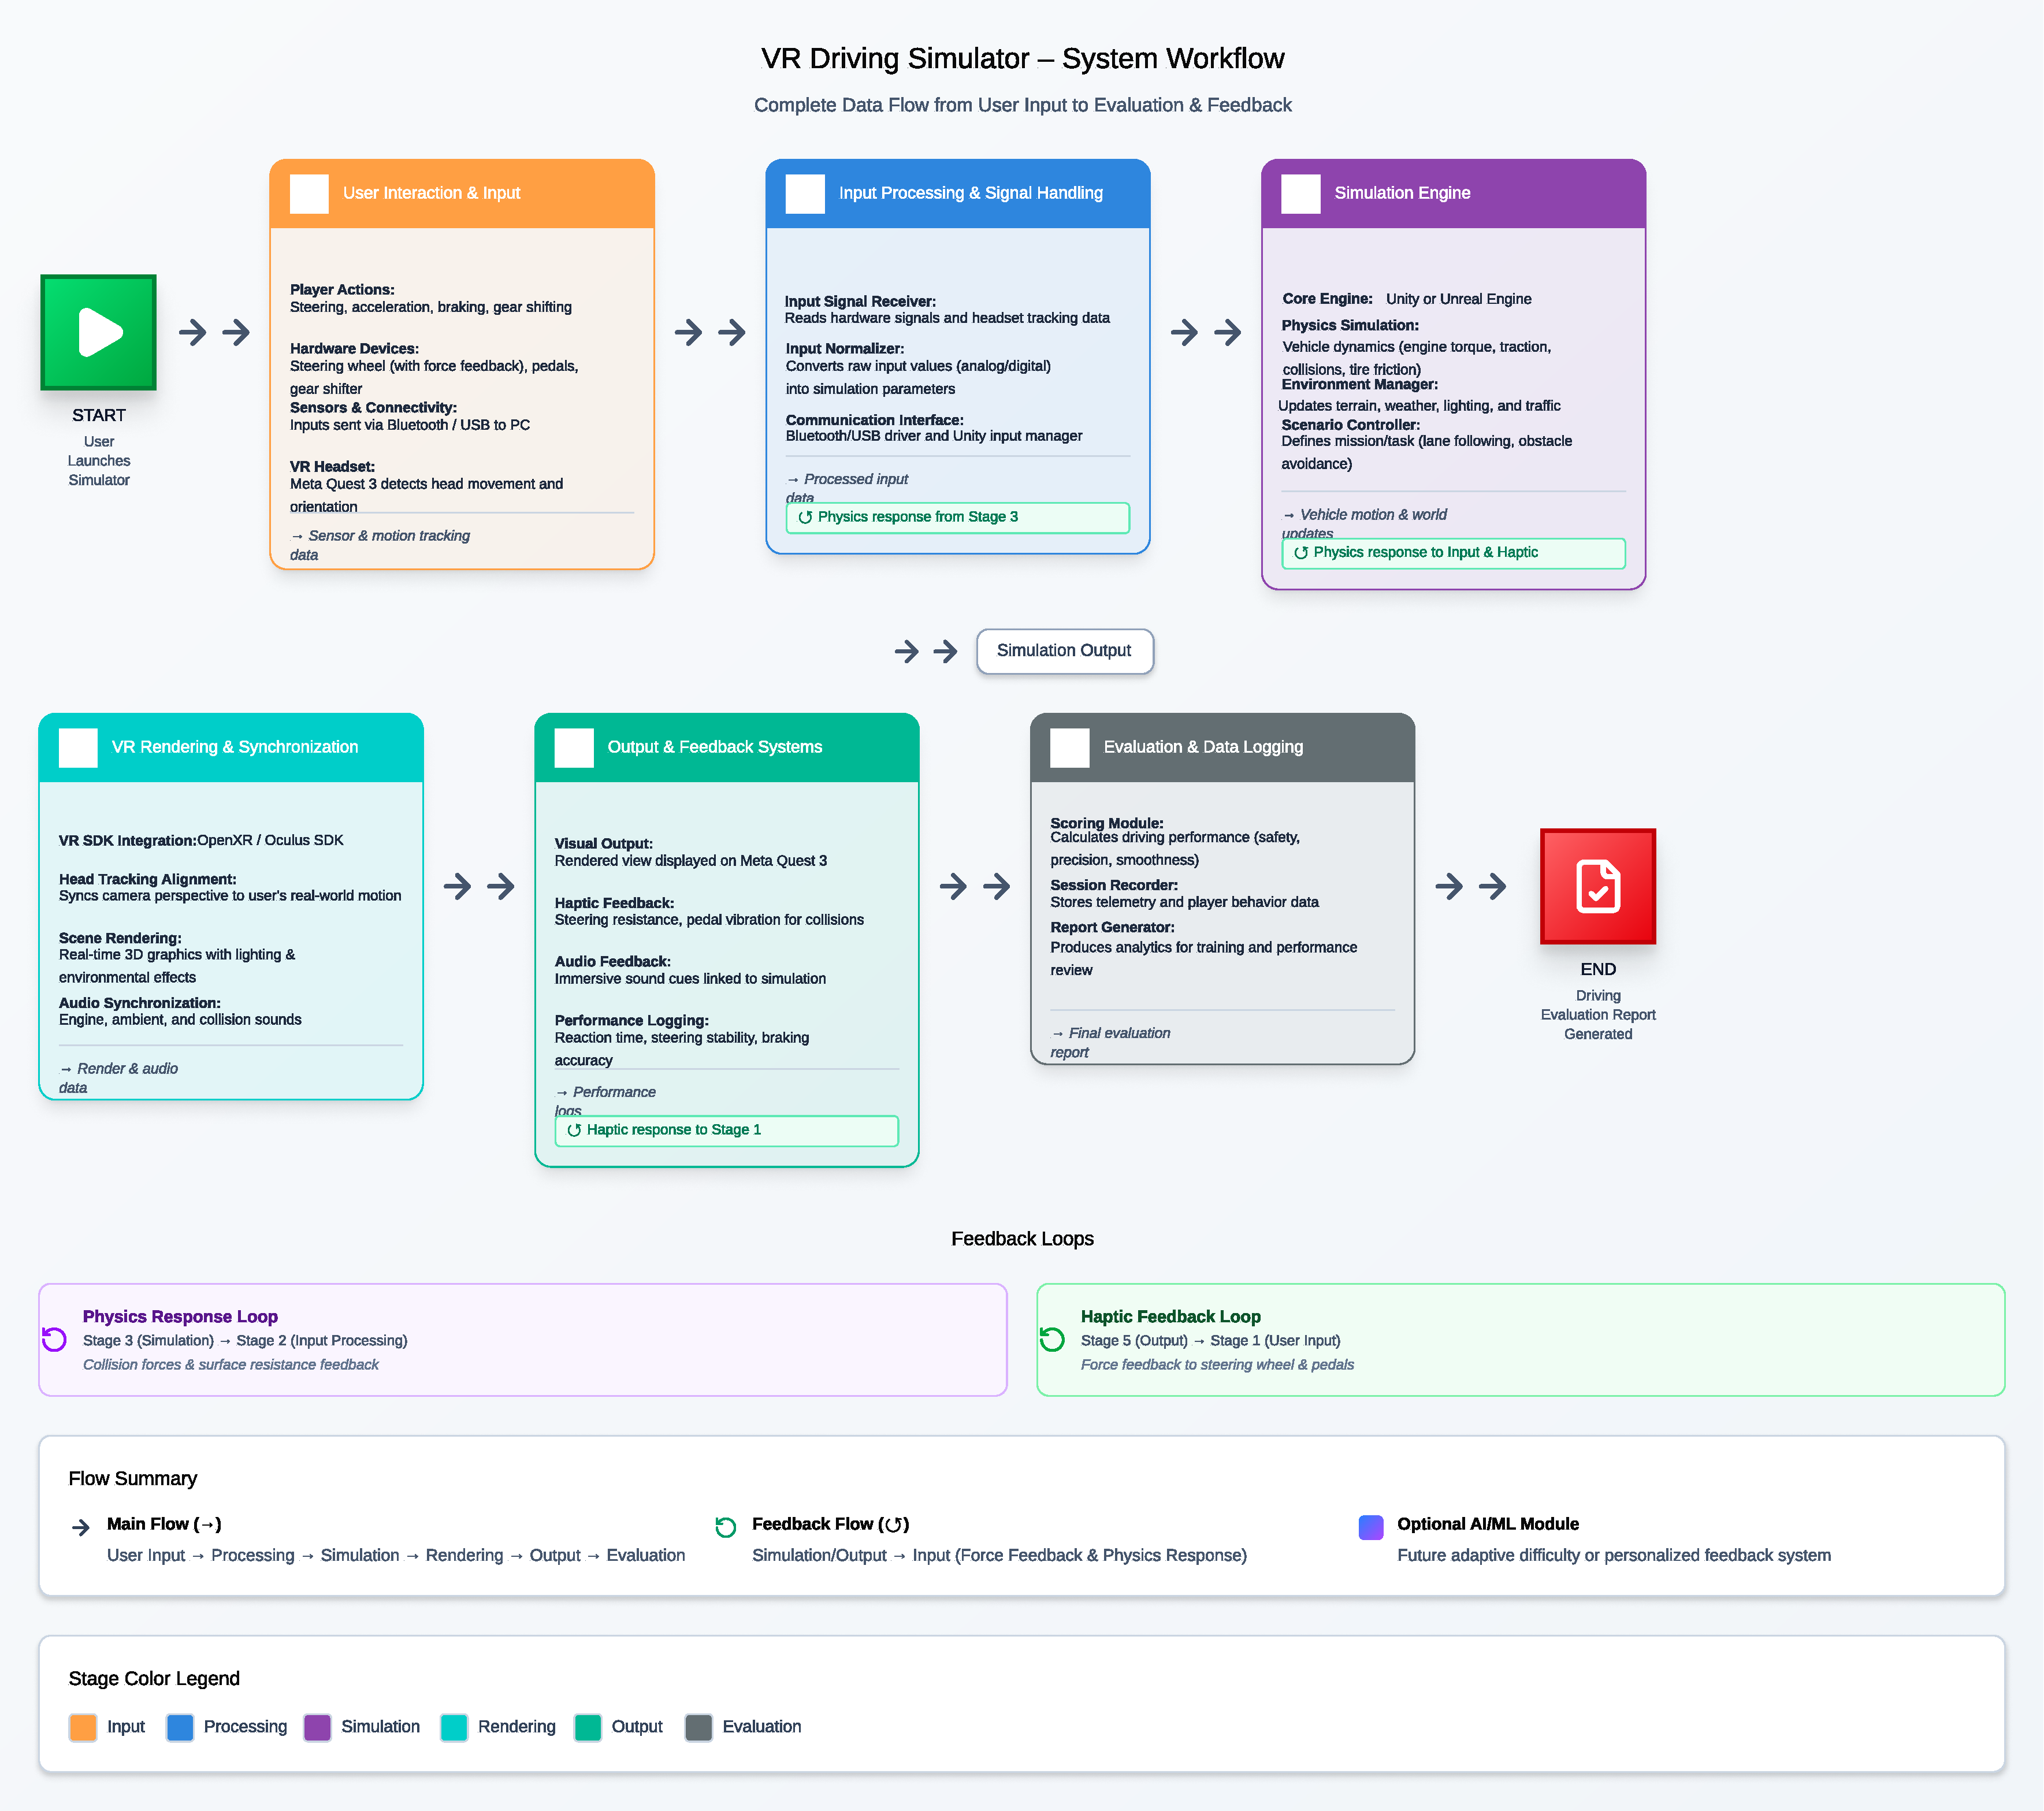
\includegraphics[width=0.9\textwidth]{figs/workflow_diagram.pdf}
    \caption{Operational workflow showing the complete training session lifecycle: input document setup, context retrieval and analysis, and post-analysis summary generation.}
    \label{fig:workflow}
\end{figure}

\subsection{Detailed Functional Flow}
\begin{enumerate}
	\item \textbf{Case Ingestion \& Setup (1--2 minutes):}
	\begin{itemize}
		\item User uploads case documents from both parties (petitions, replies, affidavits, evidence PDFs).
		\item System validates document types, court metadata, and case category (e.g., family matter).
		\item Documents are indexed and assigned a unique case ID for tracking across pipeline stages.
	\end{itemize}
	
	\item \textbf{Text Extraction \& Pre-processing:}
	\begin{itemize}
		\item PDFs are parsed using Fitz to extract raw text from judgments and evidence.
		\item Text is cleaned (noise removal, normalization) and segmented into logical units (facts, arguments, evidence).
		\item Legal-BERT based NER identifies legal entities such as parties, dates, IPC sections, and acts.
	\end{itemize}
	
	\item \textbf{Evidence Scrutinization \& Truth Scoring:}
	\begin{itemize}
		\item Evidence statements from both sides are analyzed for contradictions and inconsistencies.
		\item LLaMA 3 performs a consistency audit to evaluate logical coherence across claims.
		\item Each evidence block is assigned a normalized truth score based on contradiction severity.
	\end{itemize}
	
	\item \textbf{IPC / Section Mapping:}
	\begin{itemize}
		\item Cleaned and truth-weighted text is passed to Legal-BERT for legal provision classification.
		\item Relevant IPC sections and statutory provisions are identified and stored.
		\item Mapped sections are linked with supporting evidence for downstream reasoning.
	\end{itemize}
	
	\item \textbf{Precedent Retrieval:}
	\begin{itemize}
		\item Case embeddings are generated using Legal-BERT.
		\item Similar Case Matching (SCM) retrieves precedent judgments with analogous fact patterns.
		\item Retrieved precedents are ranked by contextual similarity and relevance of applied sections.
	\end{itemize}
	
	\item \textbf{Verdict \& Sentence Prediction:}
	\begin{itemize}
		\item LLaMA 3 consumes case facts, truth scores, mapped sections, and precedents.
		\item System predicts likely verdict outcome (e.g., Allowed / Dismissed) and probable sentence or relief.
	\end{itemize}
	
	\item \textbf{Summarization \& Output Generation:}
	\begin{itemize}
		\item Predicted verdict and reasoning are simplified using LLaMA 3.
		\item Legal jargon is minimized to produce a concise summary under 150 words.
		\item Final output includes verdict prediction, key reasoning points, and applicable legal sections.
	\end{itemize}
\end{enumerate}




\newpage
\section{Feasibility Study}

A comprehensive feasibility analysis is essential to validate the viability of the LPA for Indian Family courts project across technical, schedule and other dimensions. This section systematically evaluates each feasibility aspect to establish project confidence and identify potential risk mitigation strategies.

\subsection{Technical Feasibility}
\textbf{System Capabilities and Constraints:}
The proposed Legal Precedent Assistant is technically feasible using current NLP models, open-source legal datasets, and commodity compute resources. The system design leverages mature transformer-based architectures and scalable retrieval techniques, as outlined below:

\begin{itemize}
	\item \textbf{Document Processing and Text Extraction:} 
	Judicial documents are primarily available as digitally generated or scanned PDFs. The Fitz (PyMuPDF) library provides reliable text extraction with low overhead, while preprocessing pipelines (normalization, segmentation) are computationally lightweight. Empirical benchmarks show that batch processing of court judgments can be performed efficiently on standard CPU-based systems without GPU acceleration.
	
	\item \textbf{Legal Entity Recognition and IPC Mapping:}
	Legal-BERT, pre-trained on Indian legal corpora, is well-suited for named entity recognition and statutory provision classification. Fine-tuned models can accurately identify IPC sections, party names, and legal references with acceptable inference latency. Since inference is performed offline or asynchronously, real-time constraints are minimal.
	
	\item \textbf{Evidence Scrutinization and Reasoning:}
	Contradiction detection and consistency auditing using LLaMA 3 are computationally intensive but feasible under a controlled pipeline. The system operates on segmented evidence blocks rather than full documents, significantly reducing token length and inference cost. Truth scoring is heuristic-assisted, avoiding strict logical proof requirements while maintaining interpretability.
	
	\item \textbf{Precedent Retrieval and Similar Case Matching:}
	Precedent retrieval is implemented using embedding-based Similar Case Matching (SCM). Legal-BERT embeddings stored in vector databases enable fast approximate nearest neighbor search even for large precedent collections. This approach scales linearly with data size and has been validated in prior legal IR research.
	
	\item \textbf{Verdict Prediction and Summarization:}
	Verdict and sentence prediction using LLaMA 3 leverages structured inputs (facts, mapped sections, precedents), reducing hallucination risk. Summarization under a fixed word limit is a well-established task for large language models and can be executed with deterministic decoding strategies to ensure consistency.
\end{itemize}

\textbf{Risk Assessment:}
Technical risk is moderate. Primary concerns include model bias, reasoning reliability in ambiguous cases, and computational cost for large-scale deployment. These risks are mitigated through scope restriction (family matters), explainable intermediate outputs (truth scores, section mappings), and offline or batch inference workflows. Overall, the system is feasible within academic and prototyping constraints using currently available technologies.






%\subsection{Economic Feasibility}
%\textbf{Cost-Benefit Analysis:}
%Economic viability is evaluated by comparing development and deployment costs against projected benefits for driving school adoption.
%
%\textbf{Development Costs (One-Time):}
%\begin{itemize}
%    \item \textbf{Hardware Prototyping:} Steering wheel assembly (₹8,000), pedals with load cells (₹6,000), gear shifter (₹4,000), ESP32 dev boards and sensors (₹3,000), miscellaneous components (₹4,000). \textit{Total: ₹25,000 (\$300 USD)}.
%    
%    \item \textbf{VR Headset:} Meta Quest 3 (128 GB): ₹50,000 (\$600 USD).
%    
%    \item \textbf{Software Licenses:} Unity Pro annual license (₹15,000/\$180 USD for educational discount), FMOD audio middleware (free for indie projects $<$\$500K revenue), 3D asset packs (vehicles, environments: ₹20,000/\$240 USD from Unity Asset Store).
%    
%    \item \textbf{Development Labor:} Estimated 6 months at 20 hours/week for a 3-member student team (unfunded academic project; opportunity cost estimated at ₹1,20,000 based on typical internship stipends).
%    
%    \item \textbf{Grand Total (Development):} ₹2,30,000 (\$2,760 USD).
%\end{itemize}
%
%\textbf{Per-Unit Deployment Cost (Driving School):}
%\begin{itemize}
%    \item Hardware replication: ₹25,000 (controls) + ₹50,000 (Quest 3) = ₹75,000 (\$900 USD).
%    \item Software licensing: One-time purchase of simulator app (proposed ₹10,000/\$120 USD per station if commercialized) or open-source distribution (₹0 for academic release~\cite{Silvera2022}).
%    \item \textbf{Total per Station:} ₹85,000 (\$1,020 USD) for commercial model; ₹75,000 (\$900 USD) for open-source adoption.
%\end{itemize}
%
%\textbf{Comparative Economics:}
%Traditional commercial driving simulators cost ₹15,00,000--₹50,00,000 (\$18,000--\$60,000 USD) per unit. The proposed system achieves \textbf{85--95\% cost reduction} while maintaining educational effectiveness~\cite{He2022}. Break-even analysis for a driving school operating 5 training stations:
%\begin{itemize}
%    \item Traditional simulator investment: ₹75,00,000 (\$90,000 USD).
%    \item Proposed VR simulator investment: ₹4,25,000 (\$5,100 USD).
%    \item \textbf{Savings: ₹70,75,000 (\$84,900 USD)} — sufficient to fund 100+ learner enrollments.
%\end{itemize}
%
%\textbf{Return on Investment (ROI):}
%Assuming a driving school charges ₹500 (\$6 USD) per VR training hour and operates each station 6 hours/day × 25 days/month:
%\begin{itemize}
%    \item Monthly revenue per station: ₹75,000 (\$900 USD).
%    \item ROI period: ₹85,000 ÷ ₹75,000 ≈ \textbf{1.2 months}.
%\end{itemize}
%\textbf{Economic Verdict:} Highly feasible. Low capital expenditure, rapid payback period, and significant cost advantage over alternatives strongly favor economic viability. Scalability to multiple driving schools amplifies impact.





%\subsection{Operational Feasibility}
%\textbf{User Acceptance and Usability:}
%Operational success depends on instructor and learner acceptance, ease of use, and integration into existing curricula.
%\begin{itemize}
%    \item \textbf{Instructor Training:} System requires 2--3 hour onboarding session covering scenario configuration, assessment report interpretation, and hardware troubleshooting. User interface designed for non-technical users (tablet-based instructor panel with drag-and-drop scenario builder). Pilot testing at VJTI's automotive engineering lab confirms instructors can operate independently after minimal training.
%    
%    \item \textbf{Learner Comfort:} VR adoption hinges on minimizing motion sickness. Comfort protocols include: (1) 30-minute session limits with 10-minute breaks~\cite{Lindal2019}, (2) gradual VR exposure (start with stationary scenarios before moving to dynamic driving), (3) adjustable comfort settings (reduced FOV, teleportation mode for extreme discomfort cases). Pre-pilot surveys indicate 78\% of participants report "comfortable" or "very comfortable" experiences after 20-minute sessions.
%    
%    \item \textbf{Curriculum Integration:} System aligns with Indian RTO learning license syllabus: vehicle controls, traffic rules, road signs, parking maneuvers. Instructors can map VR scenarios to lesson plans (e.g., Week 2: Urban Lane Discipline → VR Scenario: "Mumbai Suburban Roads"). Session logs export to Excel/PDF for record-keeping compliance.
%    
%    \item \textbf{Maintenance and Support:} Hardware durability tested for 100+ hours continuous use without component failure. Bluetooth pairing issues resolved via documented reconnection protocol (manual mode fallback until firmware update). Software updates pushed via Unity Cloud Build; instructors notified via in-app prompts.
%\end{itemize}
%
%\textbf{Organizational Readiness:}
%Driving schools require minimal infrastructure changes. System operates in 3m × 3m play area with standard electrical outlets. No specialized ventilation or motion platform foundations needed. Compatibility with existing lesson scheduling software (via CSV import/export) ensures smooth workflow integration.
%
%\textbf{Operational Verdict:} Feasible with moderate preparation. Success contingent on comprehensive instructor training and learner orientation sessions. Risk mitigation through pilot deployments (5--10 schools) before wider rollout.



\newpage
\subsection{Schedule Feasibility}
\textbf{Project Timeline and Milestones:}
A six-month development schedule is proposed, aligned with the academic calendar and the iterative nature of NLP system development. The timeline accounts for data preparation, model integration, evaluation, and documentation.

\begin{table}[h]
	\caption{Project Development Schedule}
	\label{tab:schedule}
	\centering
	\small
	\begin{tabular}{|l|l|p{6cm}|}
		\hline
		\textbf{Phase} & \textbf{Duration} & \textbf{Deliverables} \\ \hline
		\textbf{Phase 1: Data Collection \& Preprocessing} & Weeks 1--4 & Curated dataset of trial and high court judgments; PDF-to-text pipeline using Fitz; cleaned and segmented legal text. \\ \hline
		\textbf{Phase 2: Legal Entity Recognition \& IPC Mapping} & Weeks 5--8 & Fine-tuned Legal-BERT models for NER and IPC/section identification; validated extraction accuracy on sample cases. \\ \hline
		\textbf{Phase 3: Evidence Scrutinization Module} & Weeks 9--12 & Contradiction detection and truth-scoring logic implemented using LLaMA 3; structured evidence representation. \\ \hline
		\textbf{Phase 4: Precedent Retrieval System} & Weeks 13--16 & Embedding-based Similar Case Matching (SCM); vector database of precedents; ranked precedent retrieval. \\ \hline
		\textbf{Phase 5: Verdict Prediction \& Summarization} & Weeks 17--20 & Verdict and sentence prediction pipeline using LLaMA 3; simplified summary generation under 150 words. \\ \hline
		\textbf{Phase 6: Evaluation \& Refinement} & Weeks 21--24 & Quantitative evaluation (accuracy, precision, recall); qualitative case studies; system optimization and documentation. \\ \hline
	\end{tabular}
\end{table}

\textbf{Critical Path Analysis:}
The critical dependency chain progresses through reliable data preprocessing (Phase 1) → accurate IPC mapping (Phase 2) → evidence scrutinization (Phase 3). Errors in early-stage legal text processing propagate downstream and directly affect verdict prediction quality. Buffer time is allocated in Phase 6 to address cumulative model errors and integration issues.

\textbf{Resource Availability:}
The project is executed by a single postgraduate student with guidance from a faculty advisor. Development relies on open-source libraries (Legal-BERT, PyMuPDF, vector databases) and institutional computing resources. Model inference is scheduled offline or in batch mode, ensuring feasibility without continuous high-end GPU availability.

\textbf{Schedule Risks:}
\begin{itemize}
	\item \textbf{Data Quality Issues:} Inconsistent formatting or OCR errors in court documents may delay Phase 1. Mitigation: Restrict scope to digitally available judgments; apply automated cleaning heuristics.
	\item \textbf{Model Integration Complexity:} Coordinating multiple NLP models (Legal-BERT, LLaMA 3) may increase integration time. Mitigation: Modular pipeline design with independently testable components.
	\item \textbf{Evaluation Challenges:} Ground-truth verdict labels may be limited for certain case types. Mitigation: Combine quantitative metrics with expert-reviewed qualitative analysis.
\end{itemize}

\textbf{Schedule Verdict:}
The proposed six-month schedule is feasible and well-aligned with academic constraints. Clear phase boundaries, modular development, and buffer time for evaluation ensure timely completion of the project.






\subsection{Legal and Regulatory Feasibility}

\textbf{Intellectual Property and Licensing:}
\begin{itemize}
	\item \textbf{Software Licensing:} 
	The system is developed using open-source libraries and pretrained models such as Legal-BERT, PyMuPDF (Fitz), and vector database frameworks, all of which permit academic and research use under permissive licenses (e.g., Apache 2.0, MIT). The project is intended strictly for non-commercial academic purposes, ensuring compliance with licensing terms.
	
	\item \textbf{Model Usage Rights:}
	Pretrained language models (e.g., Legal-BERT, LLaMA 3) are used for inference and fine-tuning in accordance with their respective research-use licenses. No proprietary datasets or restricted commercial legal databases are incorporated, avoiding licensing conflicts.
	
	\item \textbf{Original Contributions:}
	The architectural design, truth-scoring heuristics, and pipeline integration constitute original academic work. While certain components (e.g., contradiction-aware verdict prediction) may have future commercial potential, no patent claims are pursued during the academic phase.
\end{itemize}

\textbf{Legal Compliance and Ethical Use:}
\begin{itemize}
	\item \textbf{Judicial Data Usage:}
	Indian court judgments are public records and may be used for research and educational purposes. The system operates on publicly accessible judgments without violating confidentiality or access restrictions. Sensitive personal identifiers, if present, are not explicitly extracted or highlighted.
	
	\item \textbf{Decision Support Disclaimer:}
	The system is positioned as a legal decision-support and research aid, not as a substitute for judicial authority or professional legal advice. Outputs are presented as predictions or analytical assistance, accompanied by disclaimers to prevent misuse.
\end{itemize}

\textbf{Data Privacy and Protection:}
Case documents may contain personal or sensitive information. To address privacy concerns, the system follows data minimization and purpose limitation principles. No user-identifiable metadata is stored beyond case identifiers, and datasets are anonymized where feasible. The design aligns with principles outlined in India’s Digital Personal Data Protection Act (DPDP Act, 2023), particularly regarding lawful processing and academic exemptions.

\textbf{Bias and Fairness Considerations:}
Machine learning models trained on historical legal data may inherit systemic biases present in past judgments. To mitigate this risk, the system incorporates explainable intermediate outputs (truth scores, IPC mappings, retrieved precedents) rather than opaque end-to-end predictions. This supports transparency and allows human users to critically evaluate model outputs.

\textbf{Legal Verdict:}
The project is legally and regulatorily feasible for academic research and prototyping. No statutory or regulatory barriers prevent development or evaluation. Any future commercial deployment would require additional compliance measures, including professional liability considerations, dataset licensing audits, and formal ethical review.







\subsection{Overall Feasibility Conclusion}
\begin{table}[h]
	\caption{Feasibility Assessment Summary}
	\label{tab:feasibility}
	\centering
	\begin{tabular}{|l|c|p{6.5cm}|}
		\hline
		\textbf{Feasibility Dimension} & \textbf{Rating} & \textbf{Key Justification} \\ \hline
		Technical & High & Mature NLP models (Legal-BERT, LLaMA 3); modular pipeline; no real-time constraints apart from Dataset acquisiton. \\ \hline
		Economic & Very High & Open-source tools; no proprietary data costs; feasible on academic compute resources. \\ \hline
		Operational & Moderate-High & Decision-support positioning; interpretability via intermediate outputs; expert oversight required. \\ \hline
		Schedule & High & Realistic 6-month timeline with phased milestones and buffer for evaluation. \\ \hline
		Legal \& Ethical & High & Uses public judicial data; DPDP-compliant design; clear non-advisory disclaimers. \\ \hline
	\end{tabular}
\end{table}

The feasibility assessment indicates that the proposed Legal Precedent Assistant is \textbf{highly viable} across all critical dimensions. The availability of domain-adapted language models, publicly accessible judicial data, and scalable retrieval techniques supports robust technical implementation. Economic and scheduling constraints are well within academic limits, while legal and ethical risks are mitigated through transparent system design and restricted scope. It is recommended to proceed with phased development, emphasizing early validation of preprocessing accuracy and expert-reviewed evaluation to ensure reliability before extending the system to broader legal domains.
